\chapter{Fundamental Knowledge \& Related Work}
\section{Fundamental Knowledge}
This section discusses the fundamental techniques and applications foundational to the construction of the proposed system, categorized into 3 pillars: 
\begin{itemize}
    \item {Natural Language Processing (NLP):} The foundational process of transforming vast volumes of raw, unstructured textual input into logical, structured 
    data formats that machine can understand. This is fundamental for document processing, reshaping all subsequent cognitive actions.
    \item {Large Language Models (LLMs)}: The core reasoning and action components of the system, responsible for interpreting user queries, orchestrating tools, and generating responses. This pillar represents the "intelligence" of the system, enabling it to perform complex tasks and adapt to user needs.
    \item {Agentic Orchestration:} The management layer responsible for coordinating specialized AI agents to execute complex, non-linear  workflows.
    \item {System Design:} The architectural blueprint that ensures scalability and robustness, utilizing clean design patterns tailored for high-stakes educational environments.
\end{itemize}
\subsection{Natural Language Processing}

Natural Language Processing (NLP) is a crucial field of study aiming to process unstructured data from documents to a structured, semantically rich representation. This process is designed to harness the full potential of complex entity-relationship paradigms, moving from raw text to machine-inferable logic. As outlined in the core objectives of language understanding, the goal is to put information into a semantically precise form that allows for further inferences.

The standard pipeline for Natural Language Processing follows the sequence:
\begin{center}
    {Information Extraction (IE) $\longrightarrow$ Knowledge Modeling $\longrightarrow$ Information Retrieval}
\end{center}

\subsubsection*{Information Extraction (IE)}
Information Extraction is the task of identifying and understanding limited, relevant portions of a text to produce a structured representation~\cite{StanfordNLP}. Its goal is to filter out linguistic noise and isolate the atomic units of knowledge. Traditional algorithms aim to extract keywords, following thế 2 methods:

\begin{itemize}
    \item {Keyword and Feature Extraction:} Utilizing dependency parsing and statistical methods (e.g., TF-IDF) to identify high-signal terms based on syntactic importance.
    \item {Named Entity Recognition (NER):} A critical sub-task used to find and classify concepts or entities (e.g., specific academic theories, formulas, or historical figures) within a text database~\cite{StanfordNLP}. This identifies the "nodes" of our future backbone.
\end{itemize}

To capture complex entities and relationships that rigid rule-based systems miss, the process relies on probabilistic modeling. The foundation of this approach is 
Tokenization, which breaks down raw text into atomic units (tokens). Statistical algorithms, such as Conditional Random Fields (CRF) or Hidden Markov Models (HMM), 
are then applied to these tokens to calculate the probability distribution of various interpretations. This allows the system to resolve linguistic ambiguities and 
predict the most likely semantic structures or labels for sequences of text.

While traditional probabilistic models logically and practically work in many usecases, they often struggle with sparse data and lack deep semantic understanding. 
Deep Learning represents a significant advancement by shifting the target towards generating Embeddings. Instead of merely calculating discrete probabilities, Deep Learning 
architectures map tokens into a continuous, high-dimensional vector space. In this embedding space, geometrically close vectors represent semantically related concepts, 
allowing the system to grasp the underlying meaning, context, and nuance of the information rather than relying solely on surface-level statistics.
\begin{figure}[H]
    \centering
    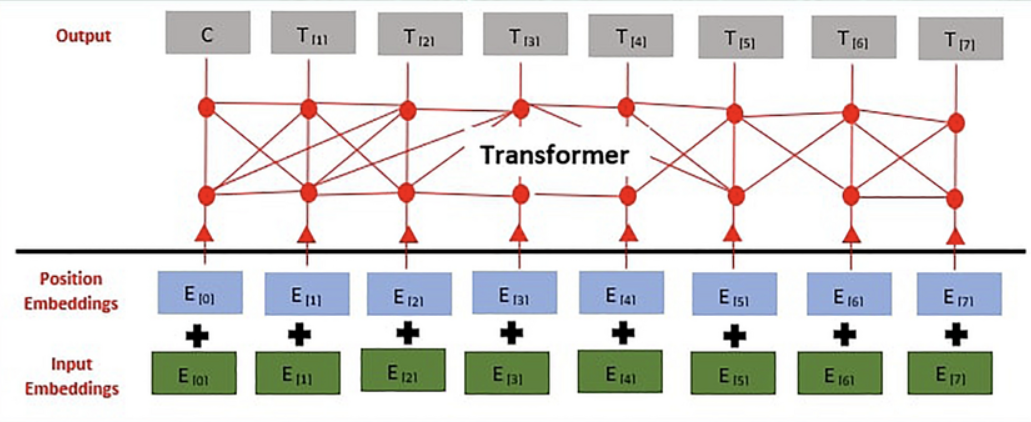
\includegraphics[width=0.7\textwidth]{Images/fundamental/embedding.png}
    \vspace{12pt}\caption{Transformer turn unstructured raw text into embeddings---numeric representation that hypothetically capture the core semantic}\label{fig:trans_embedding}
\end{figure}
The Transformer architecture was introduced, being SOTAs as well as standard method nowadays. It fundamentally change the landscape 
of NLP and enable modern Large Language Models (LLMs). The core innovation of the Transformer is the Attention Mechanism (specifically, Self-Attention). Instead of 
processing tokens sequentially, Transformers process the entire sequence simultaneously. The Attention Mechanism calculates a weighted importance score for every 
token relative to every other token in the sequence, regardless of their distance. This allows the model to instantly capture global context and long-range 
dependencies, making it the most powerful method for extracting deep, complex information from unstructured texts.

\subsubsection*{Knowledge Modeling}
Often overlooked in standard RAG systems, Knowledge Modeling is the construction stage where extracted entities are organized into a coherent structure that shapes how the system perceives and reasons.

\begin{itemize}
    \item {Semantic Parsing and Logical Form:} Mapping extracted relations into a semantically precise form, such as First-Order Predicate Calculus (FOPC) or 
    Knowledge Graphs (KG). This creates a deterministic "Backbone Graph" of the curriculum.
    \item {Embedding Space Topology:} Modeling knowledge within a continuous vector space where semantic similarity is represented by geometric proximity. 
    This allows the system to handle concepts that are conceptually related but lexically distinct.
\end{itemize}

\subsubsection*{Information Retrieval (IR)}
Information Retrieval is the active execution stage based on the result of construction phases IE and Knowledge Modeling, where the goal is to identify documents or data points relevant to a specific information need from a large document set~\cite{StanfordNLP}.

\begin{itemize}
    \item {Lexical and Keyword Matching:} Corresponding to traditional IE, this method uses exact term overlaps to find specific references or symbolic links 
    within the knowledge base.
    \item {Vector Retrieval:} the most common modern approach, utilizing the embedding space to retrieve context based on semantic similarity, typically 
    calculated via Cosine Similarity:
    \begin{equation}
        \text{similarity}(\mathbf{A}, \mathbf{B}) = \frac{\mathbf{A} \cdot \mathbf{B}}{\|\mathbf{A}\| \|\mathbf{B}\|}
    \end{equation}
    \item {The GraphRAG Paradigm:} A new powerful emerging method, where retrieval navigates the entity-relationship graph established during the modeling phase. Unlike discrete chunk retrieval, GraphRAG performs "multi-hop" reasoning to connect disparate concepts, enabling the system to resolve complex queries that require a global understanding of the educational roadmap.
\end{itemize}


\subsection{Large Language Models (LLMs)}

Large Language Models (LLMs) are deep learning-based probabilistic models trained on massive datasets to understand and generate human-like text. Mathematically, an LLM performs the task of next-token prediction by modeling the conditional probability distribution of a token $w_{t}$ given a sequence of preceding tokens $(w_{1}, w_{2}, \dots, w_{t-1})$:

\begin{equation}
P(w_{t} | w_{1}, w_{2}, \dots, w_{t-1})
\end{equation}

The structural foundation of modern LLMs is the {Transformer} architecture, which relies on the {Self-Attention} mechanism. This mechanism allows the model to compute the relative importance of different tokens in a sequence regardless of their distance. The attention score is calculated using Query ($Q$), Key ($K$), and Value ($V$) matrices derived from input embeddings:

\begin{equation}
Attention(Q, K, V) = \text{softmax}\left(\frac{QK^T}{\sqrt{d_k}}\right)V
\end{equation}

By utilizing multi-head attention and positional encoding, Transformers can capture complex linguistic patterns and long-range dependencies more effectively than previous sequential architectures like Recurrent Neural Networks (RNNs).



[Image of Transformer architecture diagram]


\subsubsection*{LLM Ecosystem: Proprietary vs Open-Weights}

The landscape of Large Language Models in the industrial layer (not research layer) is categorized by deployment strategies and the degree of architectural transparency. Closed-source and 
cloud-based models, such as GPT-4 and Claude, represent the proprietary tier of this ecosystem. These models are typically provided as a Service (SaaS), where interactions 
occur via Application Programming Interfaces (APIs) hosted on centralized, high-performance infrastructures. While these proprietary solutions consistently deliver 
state-of-the-art performance across a wide range of benchmarks, their internal mechanisms—including model weights, training datasets, and specific configurations—remain 
opaque. Furthermore, their operational use often involves per-token costs, which can become a significant factor in large-scale or iterative research applications.
\begin{figure}[H]
    \centering
    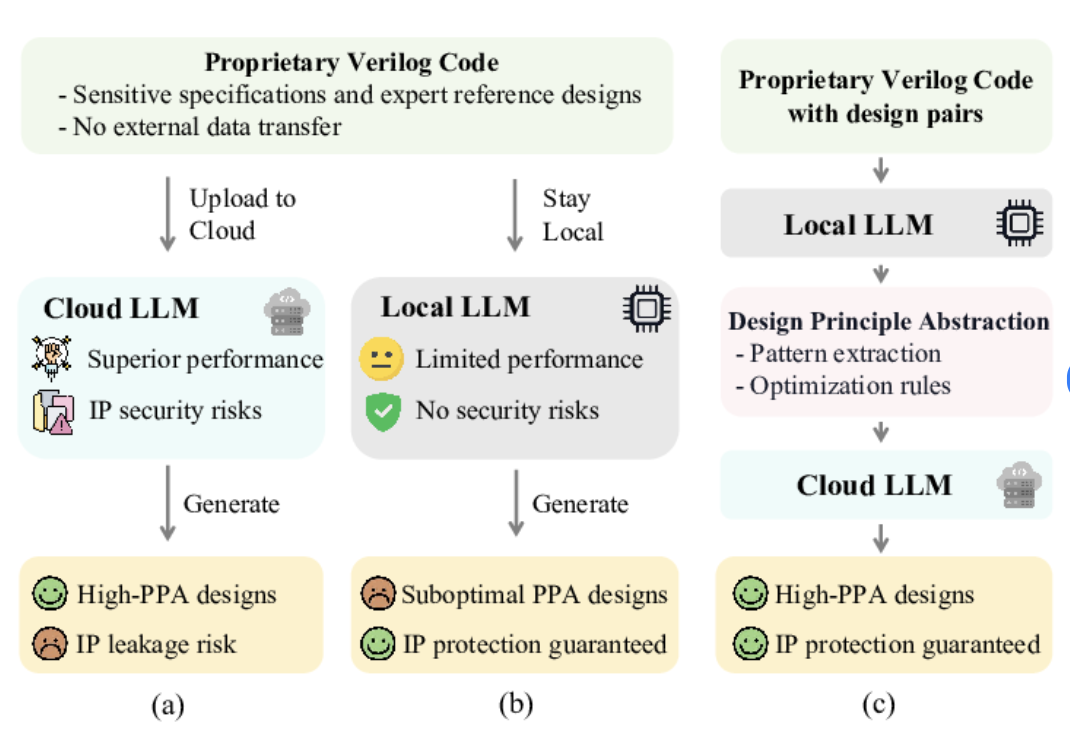
\includegraphics[width=0.7\textwidth]{Images/fundamental/cloud_local_llm.png}
    \vspace{12pt}\caption{Comparison of LLM Deployment Strategies: Traditional approaches (a) Direct cloud processing, (b) Local-only processing, and (c) Local-Cloud framework balance performance\-security without leaking IP (proposed by~\cite{IP_Safe_llm})}\label{fig:cloud_local_llm}
\end{figure}
\\
In contrast to the proprietary paradigm, the emergence of open-weights and local models has introduced a significant shift toward decentralized execution and 
architectural transparency. Initiatives such as Meta’s Llama series and Mistral release their pre-trained model parameters to the public, allowing for deployment 
on private, local infrastructures. This transparency facilitates full control over data sovereignty and privacy, as information does not need to leave the local 
environment to be processed. Consequently, these models serve as foundational baselines, providing a stable platform for both academic research and industrial 
innovation without the necessity of external API dependencies or recurring subscription fees.

Building upon these general-purpose baselines, recent advancements in the field have catalyzed a trend toward specialization, 
where models are fine-tuned or structurally modified for high-performance niche tasks. One prominent example is the development 
of coding specialists, such as Qwen-coder or CodeLlama, which are optimized specifically for source code synthesis and complex 
logical reasoning. These specialized variants often rival or even outperform significantly larger general-purpose models in 
programming-centric contexts. Beyond text processing, research has also extended these baseline architectures into the multimodal 
and generative domains. By integrating vision encoders for visual comprehension or combining LLM backbones with diffusion-based architectures, researchers have developed sophisticated models capable of high-fidelity image generation and cross-modal reasoning.

\subsubsection*{LLM Inference}

This subsection explains the utility of LLM inference parameters in controlling the generation process. During inference, the next-token probability distribution predicted by the model can be dynamically altered to balance determinism and creativity.

\paragraph*{Temperature}
Temperature ($\tau$) controls the sharpness or randomness of the predicted probability distribution. Given the logits $z_i$ output by the final layer, the adjusted probability $P(w_i)$ for each candidate token is computed using the modified softmax function:
\begin{equation}
P(w_i) = \frac{\exp(z_i / \tau)}{\sum_{j} \exp(z_j / \tau)}
\end{equation}
A lower temperature ($\tau < 1$) sharpens the distribution, making the model more confident in its top choices and producing highly deterministic text, which is ideal for rigid tasks like JSON extraction. A higher temperature ($\tau > 1$) flattens the distribution, encouraging diversity and creativity.

\paragraph*{Top-k Sampling}
Top-$k$ sampling restricts the model from considering the entire vocabulary, instead keeping only the $k$ highest-probability candidates. This approach is conceptually similar to beam search, where only the most promising paths are kept active:
\begin{equation}
V_k = \mathop{\mathrm{arg\,max}}\limits_{V' \subset V, |V'|=k} \sum_{w \in V'} P(w)
\end{equation}
The probability mass is then redistributed among these $k$ tokens. This truncation prevents the model from generating highly improbable and potentially nonsensical words (the "long tail" of the distribution).

\paragraph*{Top-p (Nucleus) Sampling}
Top-$p$ (nucleus) sampling provides a dynamic alternative to Top-$k$. Instead of keeping a fixed number of tokens, it keeps the smallest prefix subset of the vocabulary whose cumulative probability mass meets or exceeds a threshold $p$:
\begin{equation}
\min \left\{ |V'| : V' \subset V, \sum_{w \in V'} P(w) \geq p \right\}
\end{equation}
This allows the candidate pool to expand or contract organically based on the model's confidence. When the model is very confident, the nucleus contains only a few tokens; when uncertain, the nucleus expands to include more options.

\paragraph*{Repetition Penalty}
Repetition penalty modifies the logits of tokens that have already appeared in the generated sequence, mathematically reducing their likelihood of being selected again. This is crucial for preventing the model from entering infinite generation loops or excessively repeating specific phrases, ensuring a more natural and progressive text flow.


\subsection{Agentic Systems}

\subsubsection*{AI Agents: Definition and Capabilities}
An Artificial Intelligence (AI) Agent is a computational system capable of autonomous task execution through the dynamic design of workflows using available tools. 
AI agents can encompass a wide range of functions beyond natural language processing including decision-making, problem-solving, interacting with external environments, and performing actions.


\begin{figure}[H]
    \centering
    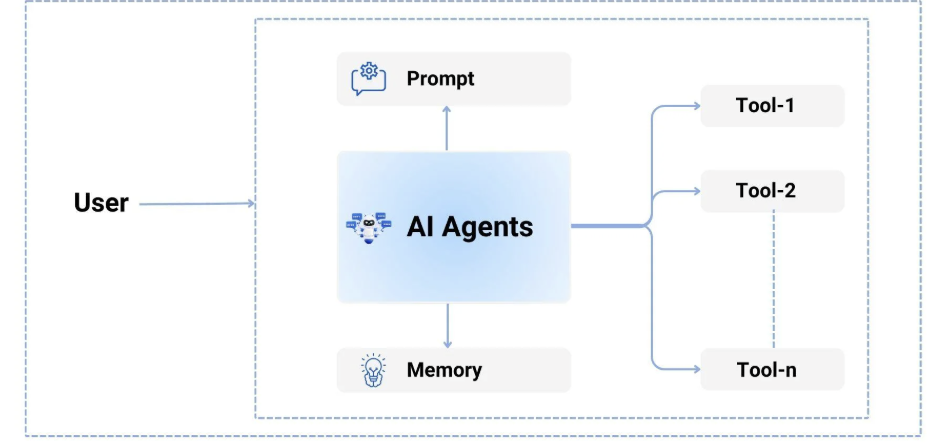
\includegraphics[width=0.6\textwidth]{Images/fundamental/agent.png}
    \vspace{12pt}\caption{Basic Single Agent diagram}\label{fig:react}
\end{figure}

Unlike Large Language Models (LLMs), which produce responses solely based on the static data used to train them and are bounded by fixed knowledge limits, agentic 
technology uses tool calling on the backend to obtain up-to-date information. They optimize workflows and create subtasks autonomously to achieve complex goals. It is 
responsible for translating high-level natural language queries into executable workflows. Instead of relying on rigid, pre-programmed paths, the agent dynamically 
analyzes the request, identifies the necessary tools, and orchestrates them in a sequence that best addresses the user's needs. This allows for a more flexible and 
adaptive system that can handle a wide variety of queries and tasks without requiring explicit programming for each scenario. 

What truly pushing agentic systems to achive what LLM can't lies in the harnessing of agentic technology. Harness is the process of constructing and integrating 
systems or infrastructure that boosts capabilities into the system. The harnessing of agentic system is critical for the agentic performance, as it enables the system 
to navigate the complex, multi-step processes required to analyze and retrieve relevant educational content based on user queries.
\paragraph*{LLM: The Logical Core}
Large Language Models (LLMs) serve as the brain of the agent, represent the thinking capability. They provide the reasoning capabilities necessary to interpret vague user queries and orchestrate the appropriate tools to find answers. The LLM is responsible for parsing the user's intent, identifying missing information, and deciding on the next actions. The reasoning and decision-making depend heavily on the type of LLM used. Upon studying the current industry, mainstream types of models include:
\begin{itemize}
    \item {Reasoning Models: }
Models such as OpenAI o1 or DeepSeek R1 are optimized for Chain of Thought processing. They excel at complex logical deduction and planning multi-step workflows before taking action. This makes them ideal for the planning phase, where they must decompose difficult user queries into a clear, executable plan before invoking any tools.
    \item {Function Calling Models}
Models such as GPT-4o or Claude 3.5 Sonnet are fine-tuned specifically to output structured data, such as JSON, rather than just conversational text. This capability is efficient for tool configuration and defining output formats. They are critical for the execution phase, as they can reliably select the correct tools and format the arguments precisely to query the database without syntax errors.
    \item {Multimodal Models}
    Models such as Gemini 1.5 Pro are trained with multimodal input. These models are essential in an educational content analysis context because they can natively understand both text and visual inputs. This allows the agent to process image frames directly alongside the user's text query without needing a separate description tool to translate visuals into text first.
    
    \item{Lightweight Efficiency Models}
    Smaller models like Llama 3 8B or GPT-4o-mini are faster and cheaper to run. They are perfect for narrow, repetitive tasks such as summarizing retrieved results or classifying user intent, where the deep reasoning capabilities of a larger model are unnecessary. Moreover, the ability to easily train and fine-tune these models facilitates customization in the design of Agentic systems.
\end{itemize}



\paragraph*{Context Engineering}
Context engineering, represent the memorization capacity, involves crafting the environment in which the LLM operates to ensure accurate and consistent outputs. This field includes several topics that govern how the model interacts with data and users.
\begin{itemize} 

\item {Prompting Strategies}
Prompting is the primary method to instruct the agent, helping it understand the goals and constraints it is dealing with. Techniques such as Query Expansion allow the agent to broaden search terms for better recall. Advanced methods like Chain of Thought (CoT) and Language of Thought (LoT) prompt the agent to articulate its reasoning process step-by-step, ensuring that complex logic is handled systematically before a final answer is generated.

\item {State Management}
To maintain a coherent interaction, systems must store chat history and the current state. This allows the agent to understand follow-up questions, such as "What happened after that?", by recalling the context of previous turns. State management ensures the agent knows exactly where it is in a multi-step retrieval process, preventing redundant actions.

\item {Retrieval-Augmented Generation (RAG)}
Agents cannot remember all the information contained in massive educational repositories, and this data is often dynamic. Retrieval-Augmented Generation (RAG) is used to retrieve external information that is not stored within the LLM's internal weights. RAG ensures the agent gets the needed information only when requested, querying the vector database to fetch relevant lecture segments or metadata to ground its answers in factual evidence.
\end{itemize}
\paragraph*{Tool Integration}
Represent the action capacity, tool integration is the process of connecting external resources (systems, software, hardware) or APIs to the agent, allowing it to perform specific functions that 
are beyond the capabilities of the LLM alone. This is critical for a automated system, as it enables the agent to interact and manipulate data in real-time. This helps 
agent 
truly integrate with the external world, understand its mission from practice instead of static texts, while also pose significant threats of misuse, when agent cause 
real life mistake and fail to judge. The key to effective tool integration is ensuring that the agent can seamlessly call these tools with the correct parameters and interpret their outputs correctly to inform its next steps.

\subsubsection*{Agent Frameworks}
The concept of an Agentic Framework arises from a practical necessity: building reliable autonomous systems requires more than just smart models; it requires a strong structure. Retraining Large Language Models to handle every specific rule or task is extremely expensive and inefficient. Therefore, the industry has shifted towards Agent Frameworks—software architectures designed to control and improve the behavior of AI without changing the model itself.

These frameworks act as a bridge, connecting the creative nature of AI with the reliable logic of software architecture. The Agents are far more than LLMs with tools and context injection; they are intelligent systems with LLMs as the neural core and architecture following software logic. Modern frameworks leverage three main aspects in Agentic design and orchestration:

\paragraph*{{Multi-agent Orchestration}} 
In complex operations, giving a single agent too much information and too many different tasks often causes errors. A single agent has a limited attention span and context window. Frameworks solve this by using Multi-agent Systems. By breaking a large job into smaller parts handled by different agents, developers can assign specific agents to each task—one for visual analysis, one for audio processing, and one for synthesis—ensuring each agent stays focused and accurate.

\paragraph*{{Agent Memorization}}
Intelligent systems need to remember information over time, but standard LLM treat every question as a new conversation (stateless). Frameworks solve this by building efficient memory systems with hierarchy, often using classes like Session or Memory. These classes act as data handlers containing multiple attributes and methods to help Agents interact with memory to retrieve previous context during run-time. Memory management almost always follows these paradigms:
\begin{itemize}
    \item {Structured Memory:} Information is organized in a structured way, allowing the system to access relevant context precisely without overwhelming the agent with irrelevant details.
    \item {Context Window Optimization:} Frameworks implement strategies to optimize the context window. The memory is connected to an external database (usually MySQL) and agentic system get needed context through lazy memory loading of tool results, conversation topics, e.t.c., perform dynamic pruning and memory injection, ensuring that the agent has access to the most relevant information without exceeding its limits, as well as saving computational resources.
\end{itemize}

\paragraph*{{Tool Abstraction}}
Frameworks turn standard code functions into Tools that agents can use on their own. The key difference between a normal function and a Tool lies in its data structure: 
\begin{itemize}
    \item {Description:} instructions on what it does and when to use it. The agent read this description when needed, doesn't overflow itself about the internal logic in the orchestration.
    \item {Input/Output Schema:} a defined structure for the input and output parameters, often in JSON format, that specifies the type and format of data the tool expects and returns. This allows the agent to understand how to call the tool correctly.
    \item {Logging memory:} functions results, errors logged into memory for agent inference, context injection and debugging.
\end{itemize}

This allows the framework to give the AI the right capabilities—like a calculator or a database search—allowing the agent to interact with the real world.
Good tool design is critical for the performance of the agentic system, as it directly impacts the agent's ability to execute tasks effectively and efficiently. 
As such, tool design must ensure that the tools are not only functional but also easily accessible and interpretable by the agent, with clear documentation and 
error handling to facilitate smooth interactions.

\subsubsection*{Langchain and LangGraph}\label{subsub:lang_intro}
The specific usecase of a our educational system necessitate a flexible, nonlinear, more orchestrated approach. While numerous frameworks exist to harness the 
capabilities of Large Language Models (LLMs), the intricate requirements of  guidance necessitate a high-level, state-aware framework.

Unlike traditional chains or data-centric frameworks like LlamaIndex and SDK, LangGraph is built upon a \textit{State Graph Architecture} where the system is modeled 
as a directed graph. In this paradigm, each node represents a specialized agent or a discrete computational step, while the edges dictate the transition logic based on the system’s current state. This modularity facilitates a sophisticated level of {Localized Context Management}. Iinstead of burdening a single agent with a big context pile of conversation history, dozen of tools and various educational usecase , the system maintains a shared State object. By granting each agent access only to the specific subset of information required for its immediate task—such as the active knowledge node or the latest student response—LangGraph ensures high-precision reasoning and mitigates the risk of context dilution while maintaining an optimized prompt size.

This granular control over context directly enables {Non-linear Branching}, allowing the system to mirror the complexity of human instruction. 
Because the workflow is state-aware, the system can gracefully navigate diverse academic scenarios, utilizing cycles and conditional logic to adapt to the learner's performance. For instance, if a student demonstrates a conceptual misunderstanding, the graph can autonomously trigger a "recovery" branch to revisit foundational prerequisites before returning to the primary roadmap. This deterministic yet flexible orchestration ensures that the AI can handle multifaceted educational use cases without losing track of the student's long-term learning objectives, a feat that is statistically difficult to achieve with stateless or purely autonomous agent frameworks.
\begin{table}[H]
\centering
\small
\renewcommand{\arraystretch}{1.6} 
\begin{tabularx}{\textwidth}{@{} l p{2.5cm} p{2.5cm} X X @{}} 
\toprule
\textbf{Framework} & \textbf{Core} & \textbf{Characteristic} & \textbf{Strength in Education} & \textbf{Limitation in Education} \\ \midrule

\textbf{LlamaIndex} & 
Data-Centric: Optimizing the interface between LLMs and private data. & 
Retrieval-heavy; focus on indexing and query engines.& 
Very powerful when it comes to multistep input output manipulation of tools, LLMs and states&
Often prioritizes data retrieval over complex, multi-step pedagogical reasoning. \\ \hline

\textbf{LangGraph} & 
Explicit state management via cyclic graphs. Supporting edges, nodes creation making full control of logic, branching& 
\textbf{Stateful, non-linear branching} with fine-grained control& 
Suitable for complex nonlinear task, with state\-aware and context, logic localization and independence &
Branching acts as a selling point and a potential logical error, when applying complex flow to simple tasks. Most of all, due to its high level abstraction, input output of LLM get unstable\\ \hline

\textbf{Google SDK} & 
Tool-Centric: Direct, low-latency access to model capabilities. & 
Functional/Linear; focus on tool-calling and result passing. & 
Deliver stable tool results, state and worker result if the pipeline is well designed&
Becomes unstable and difficult to maintain when including branching workflows. \\ \hline

\textbf{CrewAI} & 
Role-Centric: Simulating human-like collaborative teams. & 
Autonomous, task-based collaboration between predefined roles. & 
High level, well LLM and human interaction facilitation, capable of complex workflow&
Can lack the deterministic, full control orchestration required for strict academic knowledge modeling. \\ \bottomrule
\end{tabularx}
\caption{Comparison of LLM Orchestration Frameworks}\label{tab:frameworks}
\end{table}

These survey of various frameworks highlights LangGraph as top framework for educational system. While LlamaIndex offers stable operation with full control data, 
its data-centered nature often obscures the complex logic and asynchronization required for student-teacher interaction. 
The Google Generative AI SDK, though efficient for direct tool integration, lacks the complex state-management infrastructure necessary to handle the unstable nature of 
complex workflow, comparing to predecessor framework. Ability to maintain a persistent state and manage non-linear transitions of LangGraph and CrewAI provides the 
deterministic backbone required to facilitate a truly adaptive and reliable learning experience.
\subsection{System Design}

This section elucidates the software engineering principles, architectural patterns, and technological foundations utilized to construct the 
proposed system. Given the integration of high-latency AI inference with real-time educational interactions, the design strictly prioritizes modularity, 
robust state management, and horizontal scalability. Specifically, it focuses on adapting traditional paradigms to handle the non-deterministic and asynchronous 
nature of Large Language Model (LLM) orchestration and heavy multimedia processing workflows.

\subsubsection*{Software Paradigm: Object-Oriented Programming}
Object-Oriented Programming (OOP) is a programming paradigm based on the concept of "objects" which can contain data in the form of fields (attributes) and code in the form of procedures (methods). In this paradigm, computer programs are designed by making them out of objects that interact with one another. Fundamentally, this paradigm relies on four core concepts:
\begin{itemize}
    \item Class: A blueprint or template for creating objects, defining the initial state and behavior.
    \item Object: A specific instance of a class, representing a concrete entity within the system memory.
    \item Attribute: Variables bound to an object that represent its internal state or data.
    \item Function (Method): Procedures associated with a class that define the behaviors or actions an object can perform.
\end{itemize}
In the context of System Design, OOP is the dominant industry standard because the core components of this architecture are inherently stateful. Unlike simple functional scripts that execute and exit, system components must maintain persistent internal states—including conversation history, active tool configurations. The OOP provides the natural structural to manage this state lifecycle. The system leverages the four main pillars of OOP:

\begin{itemize}
    \item Abstraction: This allows the system to model complex entities by hiding internal implementation details and exposing only relevant operations, allowing the outside workflow logic to interact with high-level methods rather than raw data from lower components.
    
    \item Encapsulation: Groups related variables and functions into a single unit, protecting the internal state from unintended interference. This ensures that the memory of one component is strictly isolated and cannot be corrupted by the operations of another component running in parallel.

    \item Inheritance: This promotes code reusability by allowing new classes to derive properties from existing ones. We utilize a base class to define shared logic such as error handling, logging, and connection management. Specialized classes then inherit these foundational capabilities while implementing their specific unique behaviors, significantly reducing code duplication.

    \item Polymorphism: This allows objects of different classes to be treated as objects of a common superclass. In the orchestration layer, the system can iterate through a diverse list of components—such as different retrieval engines or analysis modules—and trigger their execution loops using a uniform interface. The orchestrator does not need to know the specific type of component it is invoking, only that every component adheres to the expected interface contract.
\end{itemize}

\subsubsection*{System Architecture: Microservices and Modular Monolithic}

System architecture defines the overall structure of a software system, organizing its major components and how they communicate. Major applications start with 
a {Modular Monolithic Architecture}. Unlike a traditional monolith where code is heavily tangled, a modular monolith compiles the application as a single 
unified program but keeps clear logical boundaries between different functions. This approach offers practical early-stage benefits: it simplifies deployment, 
ensures fast internal communication, and makes the codebase easier to test and debug.
\begin{figure}[H]
    \centering
    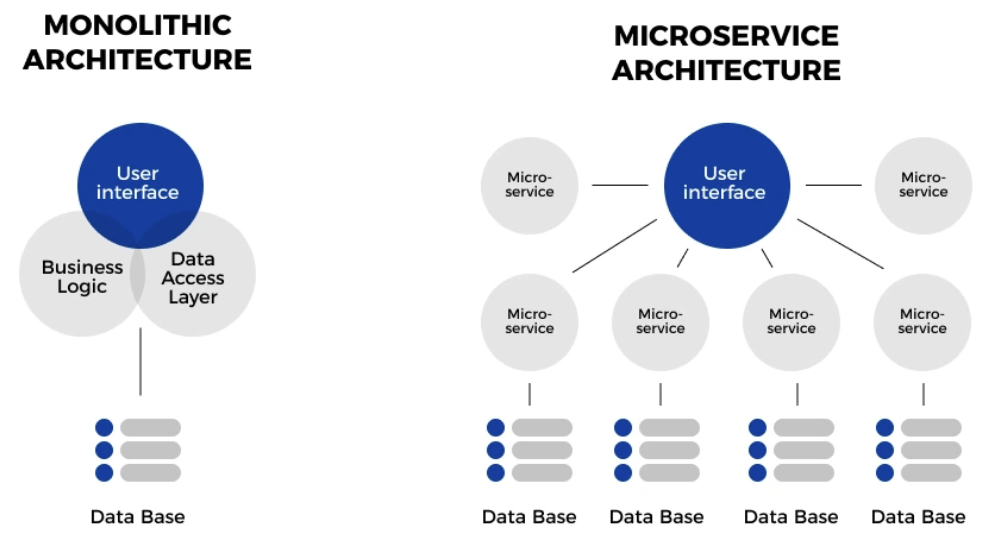
\includegraphics[width=0.7\textwidth]{Images/fundamental/micro.png}
    \vspace{12pt}\caption{Comparison of Microservice and Monolithic architecture}\label{fig:micro_vs_mono}
\end{figure}


However, as system demands grow, combining heavy processing tasks with basic web routing in a single program can cause performance bottlenecks. 
Microservices take the next step by turning logical modules into physical, independent services. Each service runs in its own process, 
often with its own separate database, and communicates with other services using standard protocols like REST APIs or message brokers.

Therefore, the Microservices architecture inherits the organizational advantages of the Modular Monolith, while providing several additional merits:
\begin{itemize}
    \item {Independent Scalability:} Microservices allow different parts of the system to scale separately. For example, a heavy processing service can be upgraded with more computing power or duplicated without needing to scale the lightweight web server. This ensures efficient hardware use during high traffic.
    
    \item {Fault Isolation:} In a microservices system, software failures are contained. If a heavy processing service crashes due to memory limits, it does not bring down the entire system. Other services, such as user login and basic web browsing, remain fully operational while the crashed service restarts.
    
    \item {Technology Flexibility:} Microservices allow developers to choose the best programming language or tool for each specific task. For instance, data science components can be built using Python for its machine learning libraries, while high-speed API routing can be written in Go or Node.js.
\end{itemize}

Alongside these benefits, Microservices possess some intrinsic disadvantages:

\begin{itemize}
    \item {Network Latency:} Internal function calls in a monolith are extremely fast. In microservices, these are replaced by network requests over the internet or local network, which inherently adds delay and processing overhead.
    \item {Operational Complexity:} Managing, monitoring, and deploying multiple independent services with separate databases is significantly harder than deploying a single program. It also requires complex strategies to keep data consistent across the entire network.
\end{itemize}

\subsection{Technology Stack and Frameworks}
The selection of frameworks is driven by the need for high-performance Python execution and seamless integration with AI libraries. These frameworks are chosen to 
building block for the implementation of the application layer, providing the necessary tools and abstractions to manage the complex interactions between the backend, frontend, and AI components. 
\subsubsection*{Backend Development}
Backend development serves as the foundational logic of any software application, responsible for data processing, security, and the orchestration of communication between the database and the client. It handles the business logic that users do not see but rely upon for functionality. For an intelligent educational system involving heavy AI workloads, the backend must be capable of handling high-concurrency requests without latency, ensuring that the complex computations of the agents do not block the user experience.
\begin{figure}[H]
    \centering
    
\includegraphics[width=0.4\textwidth]{Images/system/backend/fastapi.png}
\end{figure}
To address these requirements, we utilize FastAPI, a modern web framework for building APIs with Python. While older frameworks like Django were built on synchronous standards known as WSGI, FastAPI adopts the Asynchronous Server Gateway Interface (ASGI). This approach allows the server to handle asynchronous code natively using Python's await syntax. This represents a paradigm shift for AI applications, moving away from blocking, sequential request handling to a concurrent model where I/O-bound tasks—such as waiting for an LLM response or a database query—release the CPU to handle other incoming requests, offering some key features:
\begin{itemize}
    \item High Concurrency: By utilizing the ASGI standard, FastAPI can handle thousands of simultaneous connections (such as multiple users uploading videos or chatting with agents) without the blocking issues inherent in traditional synchronous frameworks.
    \item Data Validation: It integrates tightly with Pydantic, a data validation library. This ensures that the complex JSON outputs generated by AI agents are rigorously validated against strict schemas before being sent to the frontend, preventing runtime type errors.
    \item Performance: Built on top of Starlette, FastAPI offers execution speeds comparable to compiled languages like Go, which is critical for minimizing the latency overhead in the educational content processing pipeline.
\end{itemize}

\subsubsection*{UV: High-Performance Package Management}
Traditional Python dependency management with pip and virtualenv introduces significant overhead in complex AI projects, where dependency resolution across dozens of GPU-accelerated libraries can take several minutes. The system adopts {uv}, a Rust-based Python package manager developed by Astral, which consolidates virtual environment creation, dependency resolution, and lockfile generation into a single binary.
\begin{figure}[H]
    \centering
    
\includegraphics[width=0.4\textwidth]{Images/system/backend/uv.png}
\end{figure}
UV achieves dependency resolution 10--100 times faster than pip by implementing a custom resolver in Rust. Its deterministic lockfile mechanism ensures that all 
team members and deployment environments operate with identical dependency versions, eliminating the ``works on my machine'' class of bugs. For this project, uv manages all backend dependencies---including LangChain, LangGraph, PyTorch, and the database client libraries---providing a consistent and reproducible build pipeline from development through production deployment.
\subsubsection*{Ollama: Local Model Inference and Optimization Infrastructure}

Ollama is an advanced abstraction layer designed for managing and executing LLMs on local infrastructure. It is built upon the \texttt{llama.cpp} core, providing an efficient environment for model orchestration and hardware acceleration.
\begin{figure}[H]
    \centering
    
\includegraphics[width=0.4\textwidth]{Images/system/AI/ollama.png}
\end{figure}

A critical feature of local inference is {Quantization}, the process of reducing the precision of model weights from high-bit floating-point formats (e.g., FP16 or BF16) to lower-bit integers (e.g., 4-bit or 8-bit). This technique significantly reduces the VRAM footprint and memory bandwidth requirements:

\begin{equation}
w_{q} = \text{round}\left(\frac{w}{\Delta}\right)
\end{equation}

where $w$ is the original weight and $\Delta$ is the scaling factor. Quantization enables large-scale models to run on consumer-grade hardware with minimal degradation in perplexity and reasoning capabilities.
Moreover, it utilizes the {GGUF (GPT-Generated Unified Format)}, a binary format designed for rapid model loading and efficient metadata storage. Key technical characteristics include:
\begin{itemize}
    \item {mmap Compatibility:} Allows models to be mapped directly into memory, enabling nearly instantaneous startup times.
    \item {Unified Execution:} Supports flexible memory offloading, where layers of the model can be distributed between the GPU (VRAM) and CPU (System RAM) based on available resources.
    \item {Modelfile Abstraction:} Provides a structured way to define system prompts, temperature settings, and context window sizes within a single configuration file, ensuring deterministic behavior across different local environments.
\end{itemize}

\subsubsection*{The Langchain Ecosystem}
As mentioned in Subsction~\ref{subsub:lang_intro}, Langchain~\cite{LangChain} is a powerful framework for our educational system, with State Graph Architecture. Moreover, it is one of the first and most popular agentic 
frameworks in the industry, with a large community and rich documentation. The accumulated contributions to the ecosystem and agentic research using Langchain have provided 
us with a wealth of tools and integrations:
\begin{itemize}
    \item {Pre-built Agents:} Langchain offers a variety of pre-built agents that can be easily customized for specific use cases, such as question-answering, 
    summarization, and multi-step reasoning. In 2026, it publishes DeepAgent, capable of extremely long term reasoning and complex workflow orchestration, 
    and currently leads the harnessing researching trend in the industry.
    \item {Langfuse:} Langfuse, among with Langsmith, is one of the most powerful tools for agentic system development. It provides a comprehensive observability platform for monitoring 
    and debugging agent interactions, allowing developers to trace the decision-making process of agents in real-time. This is critical for diagnosing issues in 
    complex workflows and ensuring that the system behaves as expected, making agentic operation more transparent, manageable and less error\-prone. 
    \item {Context Management:} Langchain includes built-in context management capabilities, enabling agents to maintain context across interactions and manage state effectively.
    Those includes utilities for memory management (adapting to multiple external databases), conversation history, and dynamic context injection, which are essential 
    for building complex agentic system for long interactions over time.
\end{itemize}




\subsection{Database System Design \& Management}
Database is where you store necessary information where application can read, write, update and delete via query or integrated calls or methods. In the domain of modern software 
engineering, data handling has become increasingly complex. To address this, robust architectures utilize a Polyglot Persistence strategy, utilizing distributed 
storage technologies optimized for different data modalities.

\begin{table}[H]
    \centering
    \caption{Polyglot Persistence Architecture: Strategic allocation of storage engines.}\label{tab:polyglot_db}
    \renewcommand{\arraystretch}{1.5} % Increases row height for readability
    \small % Slightly reduces font size to fit text better
    % Defines column widths: fixed width for the first two, auto-expanding (X) for the last two
    \begin{tabularx}{\textwidth}{|p{2.0cm}|p{2.0cm}|X|X|}
    \hline
    {Storage Engine} & {Data Modality} & {System Role} & {Theoretical Justification} \\
    \hline
    Relational (MySQL) & Structured Data & User Authentication, Billing, Access Logs & Enforces ACID properties for transactional integrity and supports complex relational joins for administrative analytics. \\
    \hline
    NoSQL (MongoDB) & Semi-Structured Data & Semantic Metadata, Analysis Tags, JSON Outputs & Provides schema polymorphism to handle variable outputs from different AI agents (e.g., OCR vs. Object Detection) without sparse tables. \\
    \hline
    Object Storage (MinIO) & Unstructured Binary & Lecture Materials, Educational Assets, Audio Clips & Decouples storage from compute to prevent database bloat; utilizes Erasure Coding for high-throughput parallel streaming during ingestion. \\
    \hline
    Vector Database (Milvus) & High-Dimensional Vectors & Embeddings Index, Semantic Search & Optimized for Approximate Nearest Neighbor (ANN) algorithms (e.g., HNSW), enabling efficient similarity search in latent spaces where traditional B-Tree indexing fails. \\
    \hline
    Graph Database (Neo4j) & Multi-hop Graph Data & Knowledge Graph, Prerequisite Relationships & Optimized for traversing complex relationship networks; enables recursive queries and multi-hop reasoning to connect disparate educational concepts. \\
    \hline
    \end{tabularx}
\end{table}



\subsubsection*{Relational Database (RDBMS)}
Relational Databases are mathematically founded on Set Theory and First-Order Predicate Logic. They organize data into tuples (rows) and attributes (columns) within strictly defined relations (tables). The defining characteristic of this model is the enforcement of ACID properties (Atomicity, Consistency, Isolation, Durability), which guarantees that database transactions are processed reliably.

RDBMS is typically utilized strictly for data that requires high integrity and deterministic relationships, such as User Management and Billing. It acts as the source of truth for entity relationships, enabling complex SQL JOIN operations (e.g., selecting all learning materials uploaded by a specific role within a timeframe).
The adoption of RDBMS for core administrative data offers specific advantages to system stability.
\begin{figure}[H]
    \centering
    
\includegraphics[width=0.4\textwidth]{Images/system/database/sqlite.png}
\end{figure}

MySQL is utilized as the primary Relational Database Management System. It handles core entities such as user accounts, roles, and administrative logs, ensuring that all structured interactions follow strict relational integrity.
\begin{itemize}
    \item Transactional Integrity: In a multi-user environment where credits or permissions are updated frequently, RDBMS ensures that race conditions do not occur. For instance, if a user purchases a subscription while simultaneously uploading an educational asset, the ACID properties ensure the account balance is updated accurately before the upload permission is granted.
    \item Data Normalization: By structuring data into normalized tables (e.g., Users, Roles, Logs), redundancy is minimized. This ensures that a change in a user's details is reflected system-wide instantly, without needing to update thousands of duplicate records.
    \item Complex Querying: The robust SQL engine allows administrators to perform audit trails and analytics efficiently, such as tracking system usage patterns across different user groups, which is computationally expensive in non-relational systems.
\end{itemize}

\subsubsection*{Non-Relational Database (NoSQL)}
To address the limitations of rigid RDBMS schemas, Non-Relational databases emerged, often adhering to the CAP Theorem (Consistency, Availability, Partition Tolerance). Unlike RDBMS which prioritizes strong Consistency, NoSQL databases like MongoDB often prioritize Partition Tolerance and Availability, offering a flexible schema-less design.

Document stores are typically the primary engine for storing the Semantic Metadata derived from educational content analysis. Metadata derived from curriculum analysis is highly variable; one resource might contain OCR text, while another contains only Audio Transcripts or Face Recognition data. Document stores handle these as dynamic BSON (Binary JSON) documents, allowing fields to be added on the fly without the sparse matrices typical of rigid SQL tables.

\begin{figure}[H]
    \centering
    
\includegraphics[width=0.4\textwidth]{Images/system/database/mongodb.png}
\end{figure}
MongoDB serves as the high-performance document store for managing the semi-structured metadata generated by AI agents. It allows the system to store diverse analysis results—such as transcripts, OCR results, and agentic reasoning logs—within a single, flexible schema.
\begin{itemize}
    \item Schema Agnosticism: AI agents are constantly evolving. If an "Object Detection" agent is upgraded to output new attributes (e.g., "Confidence Score" or "Bounding Box Coordinates"), Document stores allow the new data to be saved immediately without migrating the entire database schema or breaking existing application logic.
    \item Read Performance for Aggregates: In a Knowledge-QA scenario, the system needs to retrieve the Video Title, Description, Transcripts, and Vector IDs simultaneously. In an RDBMS, this might require joining multiple tables. In a NoSQL system, this data can be stored as a single nested document, allowing the application to retrieve the entire context of a lesson in a single, high-speed read operation.
    \item Horizontal Scalability: As archives grow to thousands of hours of lecture content, metadata storage requirements increase. Native sharding capability allows data to be distributed across multiple servers economically, ensuring lookup times remain low even as the dataset grows.
\end{itemize}

\subsubsection*{High-Performance Object Storage}
While RDBMS and NoSQL excel at storing alphanumeric data, they are fundamentally inefficient for storing massive binary large objects (BLOBs) like lecture recordings, leading to database bloat and performance degradation. Object Storage systems like MinIO treat data not as a file hierarchy or a table, but as discrete objects stored in a flat address space.

High-performance architectures utilize Object Storage to handle the High Volume nature of raw educational media. It utilizes Erasure Coding—a mathematical algorithm that splits data into fragments and expands them with redundant data pieces—allowing for data recovery even if multiple drives fail. This approach decouples storage from compute; the heavy educational artifacts are offloaded to Object Storage, while the databases store only the lightweight reference pointers (URLs) to these objects.

\subsubsection{MinIO: Object Storage}
\begin{figure}[H]
    \centering
    
\includegraphics[width=0.3\textwidth]{Images/system/filestorage/minio.jpg}
\end{figure}
MinIO is deployed as a high-performance, S3-compatible object storage server. It is responsible for hosting all raw multimedia assets, including lecture videos, extracted images, and audio segments used for AI training and inference.
\begin{itemize}
    \item Decoupling Storage and Compute: By separating the raw files from the metadata databases, "database bloat" is prevented. This ensures that the RDBMS remains lightweight and responsive for user queries, while the Object Store handles the heavy I/O load of content streaming.
    \item Parallel Streaming for AI Ingestion: When an Agent analyzes a lecture recording, it requires high-speed access to the file to extract frames. Object Storage supports parallelized byte-range requests, allowing the AI to read multiple parts of a media file simultaneously. This significantly reduces the time required for the ingestion and preprocessing phase compared to reading from a standard file server.
    \item Cost-Efficiency and Redundancy: Erasure Coding allows the system to survive hardware failures without data loss, while consuming less storage space than traditional replication methods. This is vital for maintaining a massive archive of media files economically.
\end{itemize}
\subsubsection*{Vector Database}
Traditional databases are designed for structured data and are inefficient for handling high-dimensional vector data generated by AI models. Vector databases are optimized for storing and querying high-dimensional vectors, which represent the semantic content of lecture segments. They utilize Approximate Nearest Neighbor (ANN) algorithms, such as Hierarchical Navigable Small World (HNSW) graphs, to enable efficient similarity search in latent spaces where traditional indexing methods fail.

The Vector Database is the backbone of the Retrieval-Augmented Generation (RAG) paradigm, allowing the system to perform semantic search based on the embeddings generated by the AI agents. When a user query is processed, it is transformed into an embedding vector, which is then compared against the vectors stored in the database to retrieve the most semantically relevant knowledge segments.
The adoption of a Vector Database is critical for enabling the advanced retrieval capabilities required for educational analysis.

Milvus is the chosen vector database engine for SmartEdu. It indexes high-dimensional embeddings generated from course documents and lecture transcripts, providing sub-second retrieval times for semantic similarity queries across millions of vectors.
\begin{itemize}
    \item Efficient Similarity Search: Traditional databases cannot efficiently query high-dimensional vectors. Vector databases provide specialized indexing structures to handle this efficiently.
    \item Scalability for Large Datasets: As the number of educational segments grows, the vector database can scale horizontally to maintain low latency for similarity searches, ensuring that retrieval times remain fast even as the dataset expands.
    \item Integration with AI Workflows: Vector databases are designed to integrate seamlessly with AI pipelines, supporting real-time insertion and retrieval of embeddings.
    \item Support for Dynamic Data: As new educational materials are ingested and analyzed, their embeddings can be added to the vector database in real-time, allowing the system to continuously evolve and improve its retrieval capabilities without downtime.
\end{itemize}

\subsubsection*{Graph Database}
While vector databases handle semantic similarity, the structural relationships between educational concepts—such as prerequisites and curriculum hierarchies—are best modeled as a graph. 

Neo4j is utilized to store the "Backbone Graph" of the knowledge base. It represents educational entities (concepts, lessons, modules) as nodes and their pedagogical relationships as directed edges. 
\begin{itemize}
    \item Multi-hop Reasoning: Unlike relational databases that require expensive JOIN operations, Neo4j allows for efficient traversal of deep relationship chains. This is critical for detecting knowledge gaps that may span multiple prerequisite levels.
    \item Cypher Query Language: The use of Cypher enables the system to express complex pedagogical patterns, such as "Find all prerequisite concepts of concept X that the student has not yet mastered," in a readable and performant manner.
    \item Dynamic Schema: The graph model allows the knowledge structure to evolve as new educational materials are added, without needing to redefine rigid table structures.
\end{itemize}

\subsubsection*{Database Management and Observation}
Managing multiple heterogeneous database engines requires a unified observation layer to ensure data consistency and facilitate debugging during development.

DbGate is an open-source, multi-database manager used as the primary dashboard for the SmartEdu infrastructure. It provides a unified web interface to inspect and manipulate data across MySQL and MongoDB instances simultaneously.
\begin{itemize}
    \item Unified Interface: Reduces the overhead of switching between multiple specialized management tools.
    \item Schema Visualizer: Helps developers understand the evolving structure of NoSQL documents and Relational tables in real-time.
    \item Query Benchmarking: Allows for testing and optimizing complex queries before they are integrated into the application's repository layer.
\end{itemize}

\subsection{Deployment and Containerization}
Deplloyment is the process of making a software application available for real applicational usage. This section discusses the deployment strategy and the use of containerization to ensure that the system can be reliably and efficiently deployed for our AI pipeline and high\-performance stacks as discussed above.
\subsubsection*{Docker}
Docker~\cite{docker_docs} is a containerization platform that enables developers to bundle applications and their required components into isolated units called {containers}. Each container acts as a lightweight, virtualized environment that includes all the necessary elements for the application to run. Because containers are portable and consistent, they work reliably across various environments such as on-premise systems, cloud platforms, and clustered infrastructures.
\begin{itemize}
    \item {Portability:} A major advantage of Docker is its strong portability. Containers package the application together with all its dependencies, making it simple to move workloads between different environments without compatibility issues. Whether running on a local machine or a cloud server, a Docker container behaves the same way, ensuring consistency throughout the development and deployment pipeline.

    \item {Isolation:} Docker provides strong isolation between applications and their dependencies. Each container operates independently, preventing interference between applications running on the same host. This isolation enhances both security and stability, especially in shared hosting environments.

    \item {Resource Efficiency:} Docker containers are more resource-efficient than traditional virtual machines. Since containers share the same operating system kernel, they consume far less memory and disk space. This allows more applications to run on a single machine, reducing hardware overhead and simplifying resource allocation.

    \item {Scalability:} Docker supports efficient scaling of applications. By using orchestration tools such as Kubernetes or Docker Swarm, developers can easily launch multiple container instances and distribute workloads as needed. This flexibility allows systems to rapidly adjust capacity to meet varying levels of demand.

    \item {Faster Development and Deployment:} Docker improves the speed and efficiency of both development and deployment processes. Developers can work in isolated, reproducible environments identical to production, minimizing integration issues. The deployment process becomes more automated, streamlined, and less prone to errors, saving significant time.
\end{itemize}
Docker has transformed modern software development by simplifying the creation, deployment, and management of services. Its emphasis on portability, isolation, 
resource efficiency, scalability, and rapid deployment makes it an indispensable tool for both development and operations teams.

\subsection{Security: OAuth 2.0 Authorization}

OAuthis a widely used authentication and authorization protocol in backend systems across various programming languages and frameworks. Here are some general benefits of incorporating OAuth into the backend system:

\begin{itemize}
    \item {Security:} OAuth provides a secure way for users to grant third-party applications limited access to their resources without sharing their credentials. This reduces the risk of unauthorized access and protects user data.

    \item {User Experience:} OAuth enables seamless authentication and authorization experiences for users by allowing them to log in to your application using their existing accounts from trusted providers. This eliminates the need for users to create and manage yet another set of credentials.

    \item {Single Sign-On (SSO):} OAuth facilitates single sign-on capabilities, enabling users to access multiple applications and services with a single set of credentials. This improves user convenience and reduces the likelihood of password fatigue.

    \item {Granular Permissions:} OAuth allows you to define and enforce granular permissions for accessing resources. This ensures that third-party applications only have access to the specific resources they need, enhancing security and privacy.

    \item {Scalability:} By offloading user authentication and authorization to OAuth providers, your backend system can better handle scalability challenges. OAuth providers are equipped to handle large volumes of authentication requests efficiently, allowing your application to scale more effectively.

    \item {Standardization:} OAuth is a widely adopted and standardized protocol, supported by major technology companies and libraries across different programming languages. Leveraging OAuth in your backend system ensures compatibility with a broad ecosystem of tools and services.

    \item {Compliance:} OAuth implementations often come with built-in support for compliance with regulatory requirements such as GDPR (General Data Protection Regulation) or HIPAA (Health Insurance Portability and Accountability Act). This can simplify your compliance efforts and reduce legal risks.
    \item {Developer Ecosystem:} OAuth has a large and active developer community, providing extensive documentation, libraries, and support for various 
    programming languages and frameworks, such as PyJWT for protocol schema, e.t.c. This makes it easier for developers to implement OAuth in their backend 
    systems and troubleshoot any issues that may arise.
\end{itemize}

\section{Related Work}

\subsection{Document-Knowledge Modeling}
    Converting documents into structured knowledge representations has become a critical task for so long in the industry and education specifically. To replace manual 
curation in educational contexts, which is time-consuming and not scalable, prior attempts have been focusing on the power of entity extraction, prerequisite relation 
reasoning, and RAG. This has been indeed a fine strategy, given the success of early supervised models like \texttt{PREREQ}~\cite{PREREQ} using latent topic 
representations with Siamese networks to infer course dependencies, which achieved over 70 \% Precision@100 scores on the \texttt{University Course} 
and \texttt{NPTEL MOOC datasets}. However, the traditional methods of entity extraction and relation reasoning often rely on rule-based systems or pure statistical machine learning techniques, 
which can struggle to capture the complexity and nuance of educational content's relationships. Moreover, recent researches~\cite{weller2025theoretical,LostInTheMiddle} have proven that models 
fail drastically to access relevant information when documents exceed a certain length. That is the reason why though prior researches gained impressive results on medium retrieval benchmarks, 
they are not easily applied in industry when it comes to massive and unstructured enterprise data.
\begin{figure}[H]
    \centering
    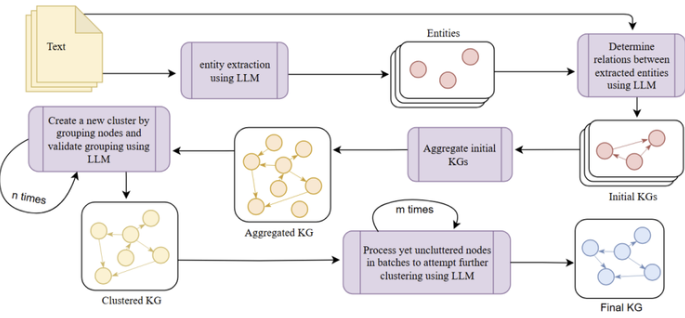
\includegraphics[width=0.8\textwidth]{Images/relate/kggen.png}
    \vspace{12pt}\caption{KGGen with multiturn LLM reasoning, grouping generation}\label{fig:kggen}
\end{figure}
    To address this, LLM-based frameworks have been widely proposed. A prime example is \texttt{KGGen}~\cite{KGGen}, an automated system that utilizes a 
clustering algorithm to group synonymous entities and relations, resulting in denser and better-connected graphs that scored an impressive 81.03\% average 
fact accuracy on the \texttt{MINE-2} (Measure of Information in Nodes and Edges) benchmark. The \texttt{EDC}~\cite{EDC} framework extends this capability by 
extracting, automatically defining schemas, and canonicalizing knowledge triples without predefined schemas, consistently surpassing state-of-the-art baselines on 
complex datasets like \texttt{WebNLG}, \texttt{REBEL}, and \texttt{Wiki-NRE}. 
\begin{figure}[H]
    \centering
    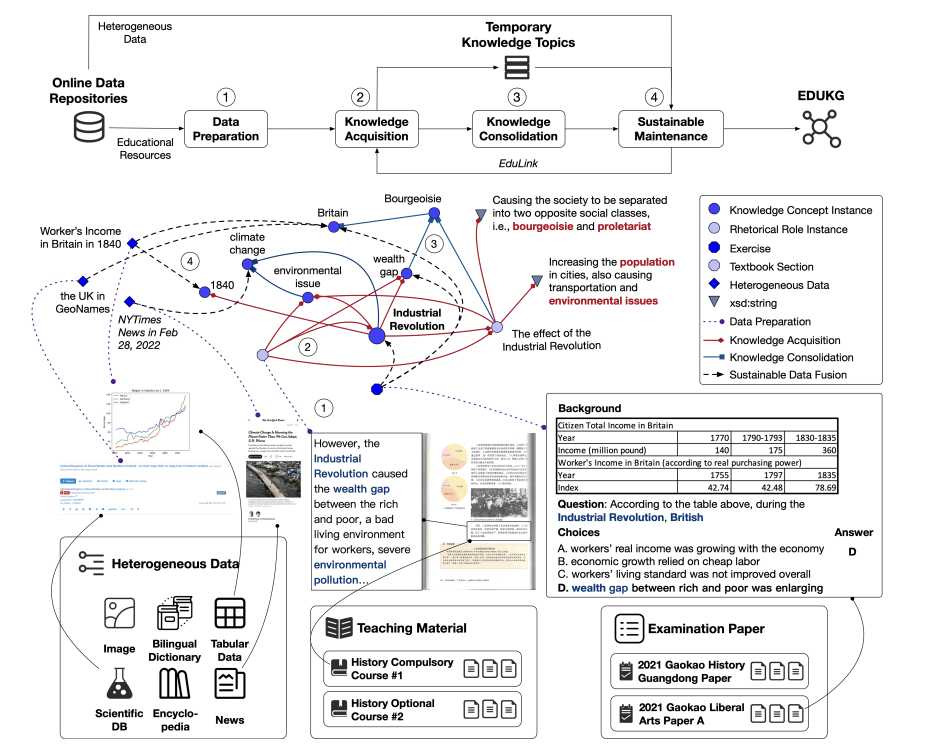
\includegraphics[width=0.8\textwidth]{Images/relate/edukg.png}
    \vspace{12pt}\caption{The end-to-end EduKGPipeline framework for educational knowledge construction and retrieval.}\label{fig:edukgpipeline}
\end{figure}
    However, LLMs have deadly drawbacks. First and most popular of all is the "hallucinations problem" leading to inaccurate, destructurized extractions. To mitigate this, \texttt{GraphJudge}~\cite{GraphJudge} proposes using a fine-tuned open-source LLM as a "judge" to score and filter out incorrect 
knowledge triples generated by naive LLMs. Validated on general (\texttt{REBEL-Sub}, \texttt{GenWiki}) and domain-specific benchmarks (\texttt{SCIERC}, 
\texttt{Re-DocRED}), it achieved over 90\% judgement accuracy. Furthermore, for large-scale educational and enterprise systems requiring cost and latency 
optimization, comprehensive hybrid pipelines have proven highly effective in practices. For instance, \texttt{EduKGPipeline}~\cite{EduKGPipe} establishes 
an end-to-end framework fusing traditional text extraction with transformer-based weighting, demonstrating high precision on educational transcripts from the 
\texttt{CCI dataset}. 
\begin{figure}[H]
    \centering
    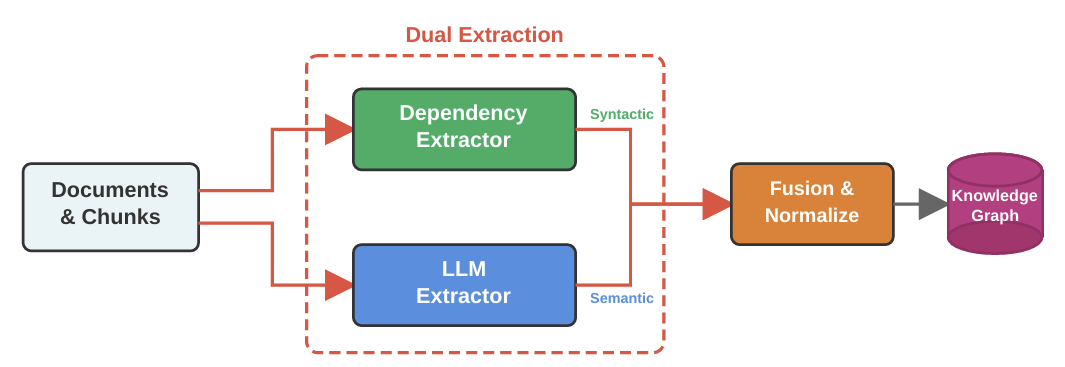
\includegraphics[width=0.8\textwidth]{Images/relate/graphrag hybrid.png}
    \vspace{12pt}\caption{Hybrid architecture of GraphRAG allow minimal cost and guarantee alignment of generated to original context}\label{fig:graph_hybrid}
\end{figure}
Similarly, recent efficient GraphRAG architectures~\cite{GraphRAG} substitute expensive LLM extractions with classical dependency parsing 
to maintain scalability, retaining 94\% of LLM-based performance on \texttt{RAGAS} metrics when evaluated on real-world enterprise datasets like \texttt{CCM} 
(Custom Code Migration). Finally, \texttt{CoDe-KG}~\cite{CoDeKG} utilizes syntactic decomposition to process complex sentences, thereby significantly enhancing 
information recall by an 8-point gain on rare relations across the \texttt{REBEL} and \texttt{WebNLG2} benchmarks.

Another inevitable error lies in the LLMs' limited context length, making it unable to generalize broad knowledge. It is good when discovering short-dependent 
context/entities/relationships in small sections but 
fails for long dependencies of extremely long documents and course information. Trying to inject an excessive amount of information even when cut by windows, 
until now with the current level, only leads to redundant costs from multiple calls, information overload, and decreased accuracy. To uncover hidden relationships 
and deduce learning paths beyond textual information, some studies shifted to an algorithmic approach.
\begin{figure}[H]
    \centering
    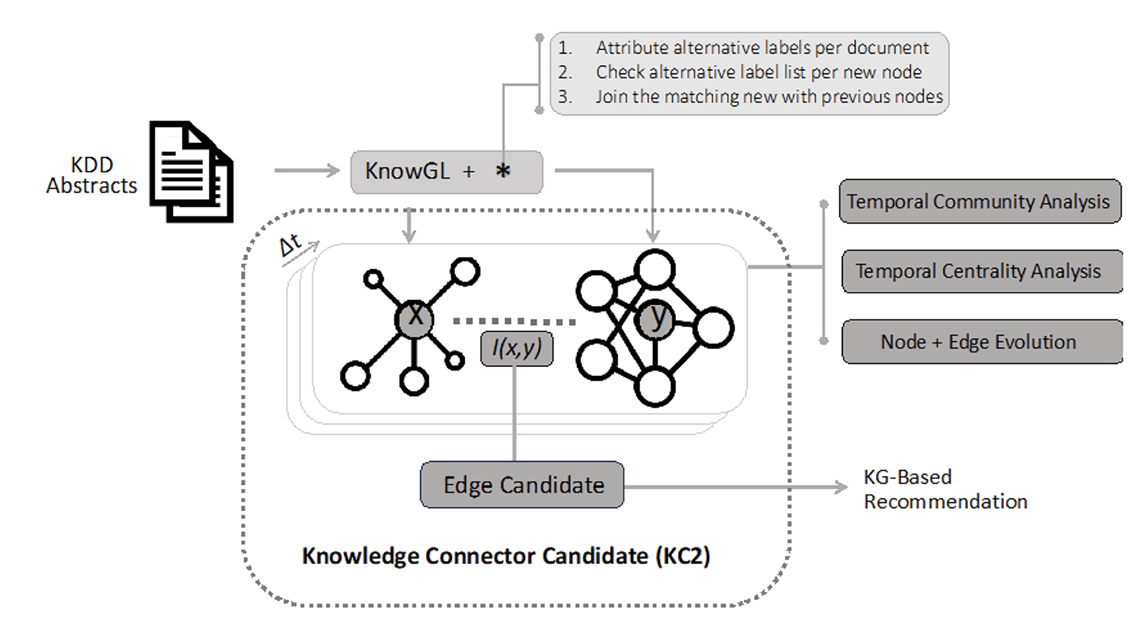
\includegraphics[width=0.8\textwidth]{Images/relate/dkg.png}
    \vspace{12pt}\caption{Dynamic Knowledge Graph (DKG) approach tracking knowledge evolution over time.}\label{fig:dkg}
\end{figure}
The \texttt{Dynamic Knowledge Graph (DKG)}~\cite{DKG} is one of the strongest representative to this approach, analyzing Knowledge Graph's macroscopic structure. To recommend strong relational paths, DKG introduces the \texttt{KC2 (Knowledge Connector Candidate)} algorithm, which uses closeness 
centrality to suggest connections between disconnected knowledge islands. Additionally, to cluster knowledge into logical chapters or modules, the 
\texttt{Leiden}~\cite{Leiden} algorithm is utilized to optimize the CPM quality function, ensuring that knowledge communities are absolutely well-connected 
and not disjointed—a common flaw of the traditional Louvain algorithm. It also divides KGs into discrete time snapshots and applies network science to track 
knowledge evolution and clustering group changes, creating a dynamic regroup, reformulation of clusters and formulation of new knowledge groups.

\subsection{Generative AI in Interactive Teaching}
Bridging the gap between raw document extraction algorithms and end-user educational platforms is the integration of Generative AI and Large Language Models (LLMs). 
The increasing accessibility and reasoning capabilities of Generative AI tools have led to widespread exploration in educational settings, fundamentally 
transforming traditional teaching and learning paradigms~\cite{AI_in_Edu}. Modern LLM agents are proved to be capable of autonomous reasoning, 
tool manipulation, and orchestrating complex academic tasks. 

\subsubsection*{Advances in Educational Agents}
Recent surveys highlight the versatility of LLM agents in automating multifaceted educational workflows, ranging from curriculum design to generating highly contextualized 
feedback~\cite{llm_in_edu}. These agents operate dynamically, leveraging multi-hop reasoning and continuous interaction to adapt to a student's cognitive state. A qualitative study involving educators demonstrated that the core impact of generative models spans three critical pillars: active teaching and learning, administrative automation, and personalized assessments~\cite{AI_in_Edu}. 

A prominent, large-scale empirical example of this shift is the integration of AI within Harvard University's CS50 course. By deploying a suite of specialized 
AI-based software, the course successfully approximated a 1:1 teacher-to-student ratio. Crucially, the system was designed with pedagogical boundaries—guiding 
students toward conceptual understanding rather than merely offering outright code solutions. This constrained autonomy proved highly effective in code explanation, 
style improvement, and administrative querying, demonstrating the practical viability of AI as a ubiquitous teaching assistant~\cite{ai_4_CS50}.

\subsubsection*{Challenges and Deployment Bottlenecks}
Despite the profound opportunities, deploying LLM agents in educational ecosystems introduces substantial systemic and ethical challenges. The inherent probabilistic 
nature of LLMs frequently leads to "hallucinations," where the model confidently generates factually incorrect or pedagogically flawed information. Furthermore, 
there is a significant risk of cognitive offloading, where students develop an overreliance on AI, thereby degrading their independent problem-solving 
skills~\cite{llm_in_edu}. 

From a practitioner's perspective, integrating these models into open-source or institutional infrastructure often encounters severe operational bottlenecks. 
Empirical analyses of LLM-based open-source projects categorize these challenges primarily into model configuration issues, connection instabilities, and feature 
misalignment, all of which hinder seamless deployment~\cite{open_source_isue}. Furthermore, theoretical analyses of LLM representations reveal phenomena such as 
"semantic collapse," where the continuous manifold of the model's activations struggles to maintain stable, logically sound ontologies over continuous, long-term 
reasoning tasks without rigid architectural constraints~\cite{semantic_collapse}. These limitations emphasize the need for robust frameworks to 
tightly navigate the semantic boundaries for AI agents in an academic context.

\subsubsection*{Agentic Workflows}
As educational AI transitions from static next-token prediction to autonomous multi-agent collaboration, ensuring the reliability, alignment, and transparency of 
these systems becomes a critical engineering challenge. Traditional benchmarks, which typically evaluate single-response accuracy, are inadequate for assessing the 
non-linear, multi-step nature of agentic workflows. 

This necessitates the development of rigorous, process-aware evaluation frameworks. Architectures like the Adaptive Evaluation Multi-Agent (AEMA) framework have been 
proposed to address this gap. AEMA provides an auditable, multi-step evaluation mechanism that operates under human oversight, ensuring that the agents' internal 
decision-making processes, tool selections, and collaborative strategies are verifiable and transparent~\cite{AEMA_agentic_eval}. Implementing such verifiable 
frameworks is essential to mitigate the risks of unconstrained autonomy, ensuring that the integration of AI into education remains both trustworthy and pedagogically effective.

\subsection{Educational Intelligent System}
Smart AI based educational systems has leverage from pure research topic and find itself introduced to commercial use. A lot of Intelligent commercial platforms have been 
born recently, and research instituitions have also propose a fully end-to-end pipeline beyond a benchmarked study method. 

In research field,~\cite{EduKG} (along with variants like K12EduKG and MOOC-KG) has been developed to uniformly model knowledge from textbooks and online courses. The~\cite{EduKGPipe} framework automates KG construction from unstructured PDF documents by extracting keywords via Keybert and performing semantic linking with LLMs. 
Furthermore, \texttt{MEduKG} pushes beyond text limitations by integrating multi-modal data into the graph, thereby enhancing the system's comprehensiveness and 
vividness for students.

As mentioned, some systems relating to this field have also reached the market. Popular platforms worldwide like \texttt{Khanmigo} leverage 
Generative LLMs to provide personalized tutoring and real-time feedback, with enormous available resources.
For Vietnamese representative, \texttt{VioEdu} utilizes a manually curated knowledge tree to structure its curriculum, while 
\texttt{EdMicro}, specialized for enterprises, employs a skill matrix to map out learning objectives and prerequisites. 
 These systems represent different approaches to integrating AI into education, each with its own strengths and limitations in terms of scalability, personalization, and content structuring.
Based on practical surveys and evaluation criteria, current educational systems in the market exhibit various characteristics regarding AI and knowledge structuring. A comparative analysis of these platforms is presented in Table \ref{tab:edu_sys}.

\begin{table}[H]
\centering
\resizebox{\textwidth}{!}{
\renewcommand{\arraystretch}{1.4}
\begin{tabular}{|p{8.0 cm}|c|c|c|c|c|}
\hline
\textbf{Criteria} & \textbf{EduKG} & \textbf{Khan Academy} & \textbf{Docebo} & \textbf{VioEdu (FPT)} & \textbf{EdMicro} \\
\hline
\textbf{Adaptive learning:} Personalize the learning process based on needs, abilities, and preferences. & High & High & Low & Medium & Medium \\
\hline
\textbf{Intelligent Recommendations:} Some personalized suggestions courses, videos based on preferences, and areas of improvement. & High & High &  & Low &  \\
\hline
\textbf{Natural language processing for queries:} Based on the questions from learners, it can give out the answer based on the content the LMS has in its DATABASE. & High & Medium & & & \\
\hline
\textbf{Learning analytics/Progress Tracking:} AI-based analytics track and analyze user progress. Can visualize using tracking board, and leaderboard. & Medium & High & High & High & High \\
\hline
\textbf{Text-to-audio content:} Provide audios for text content. & & High & & & \\
\hline
\textbf{Interactive learning method:} Interactive content, such as quizzes, coding exercises, and simulations, can engage learners and reinforce learning. & Low & Low & Medium & Medium & Medium \\
\hline
\textbf{Dynamic KG Reasoning \& Roadmap:} Automatically extract concepts and mathematically reason long-term prerequisite learning paths without manual expert input. & & & & & \\
\hline
\end{tabular}
}
\caption{Comparative analysis of representative educational intelligent systems based on key AI and knowledge features.}\label{tab:edu_sys}
\end{table}

\subsection{Conclusion and Research Gaps}\label{sub:gaps}
During the survey of mentioned representative researches, upon studying from multiple peer reviews and self-reviews of those, this report pinpoints the following core 
research gaps in the current landscape:

\paragraph*{{Limitations in Automation and Cost Optimization:}} All mentioned big systems heavily depend on manually built knowledge trees or skill matrices. Course contents, 
structured and ordered by expertise indexing, but lack inner modelling and semantic makes the system less adaptive to students' needs and preferences, 
leading to good courses recommendations but terrible inner course concept recommendations.
This makes learning path become a linear process and not flexible on the micro scale, with little to no revision and update. 
The lack of automation also limits the scalability of these systems, as manual labeling becomes increasingly impractical as the amount of content grows.
\paragraph*{{Lack of Connectivity and Transparency in Lesson Structures:}} Traditional methods like clustering in text-mining often produce disconnected 
or fragmented knowledge groups. Existing learning platforms typically lack a standard, mathematically proven network algorithm for dividing study modules, leading 
to disjointed learning path that disrupt the learners' cognitive flow.
    
\paragraph*{{Static Roadmap Reasoning and Gap Detection:}} While current LMSs and AI tutors provide generated advice, they are actually still relied on traditional long 
form docs or RAG, lacking the network structure and deterministic approach to map out prerequisites dynamically. The identification of critical "knowledge gaps" remains 
static and reactive, failing to automatically trace back to the fundamental bridge concepts (based on network centrality) that cause student bottlenecks.

So far~\cite{EduKGPipe} and its lineages have made a significant attempt to propose solutions to those mentioned problems with an 
end-to-end pipeline that fuses traditional text extraction with transformer-based weighting.~\cite{DKG} has proposed what~\cite{EduKGPipe} is missing: a mathematical 
efficient community detection method, furthermore solve the connectivity and transparency issues in lesson structures that almost all of previous pipeline encountered. 
However both have their own limitations. The former has no deterministic knowledge mapping, which causes knowledge disruption (even when the graph is not fragmented), 
while the latter pipeline is not as efficient in multistep extraction as the former, thus good for knowledge modeling and analysis but not inference and recommendation. 
Finally, a lot of great proposal here are not widely adapted due to the lack of a comprehensive system that make use of their research project. 

